% Add \usepackage{graphicx} to the LaTeX preamble.
% The PNG files are in the paper_figures/ directory.

\begin{figure}[htbp]
  \centering
  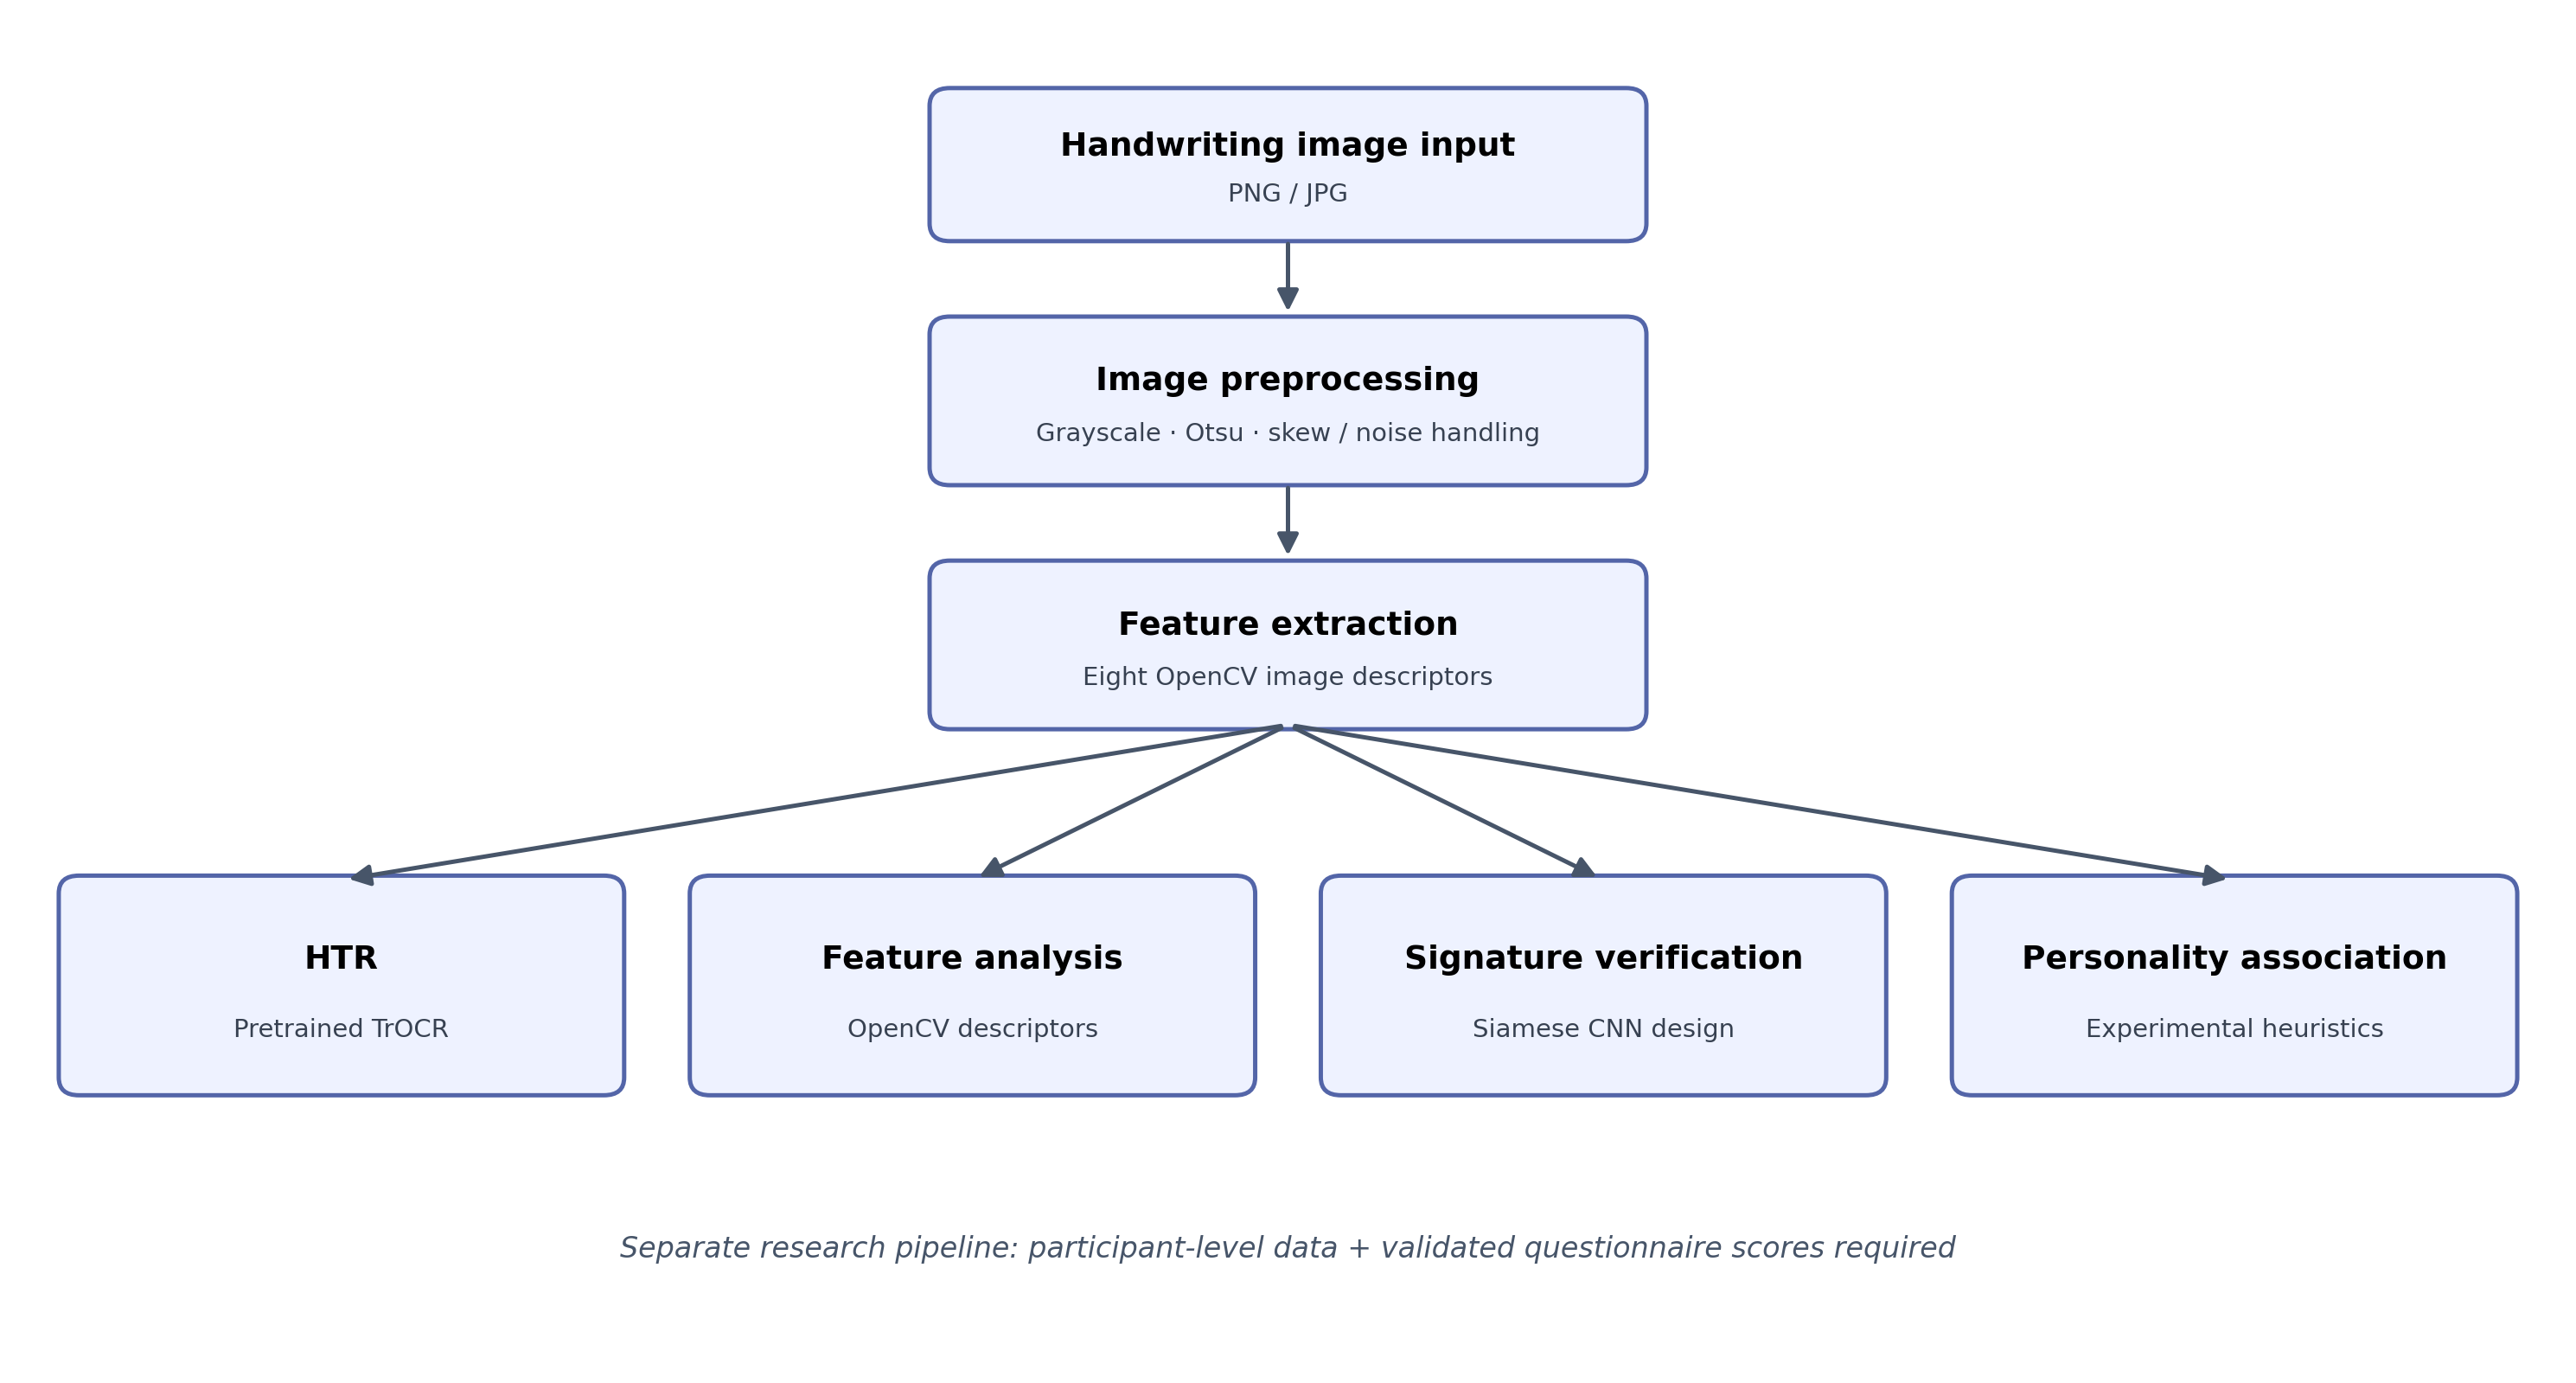
\includegraphics[width=\columnwidth]{paper_figures/fig1_architecture.png}
  \caption{Overall architecture of the GraphVision AI framework.}
  \label{fig:architecture}
\end{figure}

\begin{figure}[htbp]
  \centering
  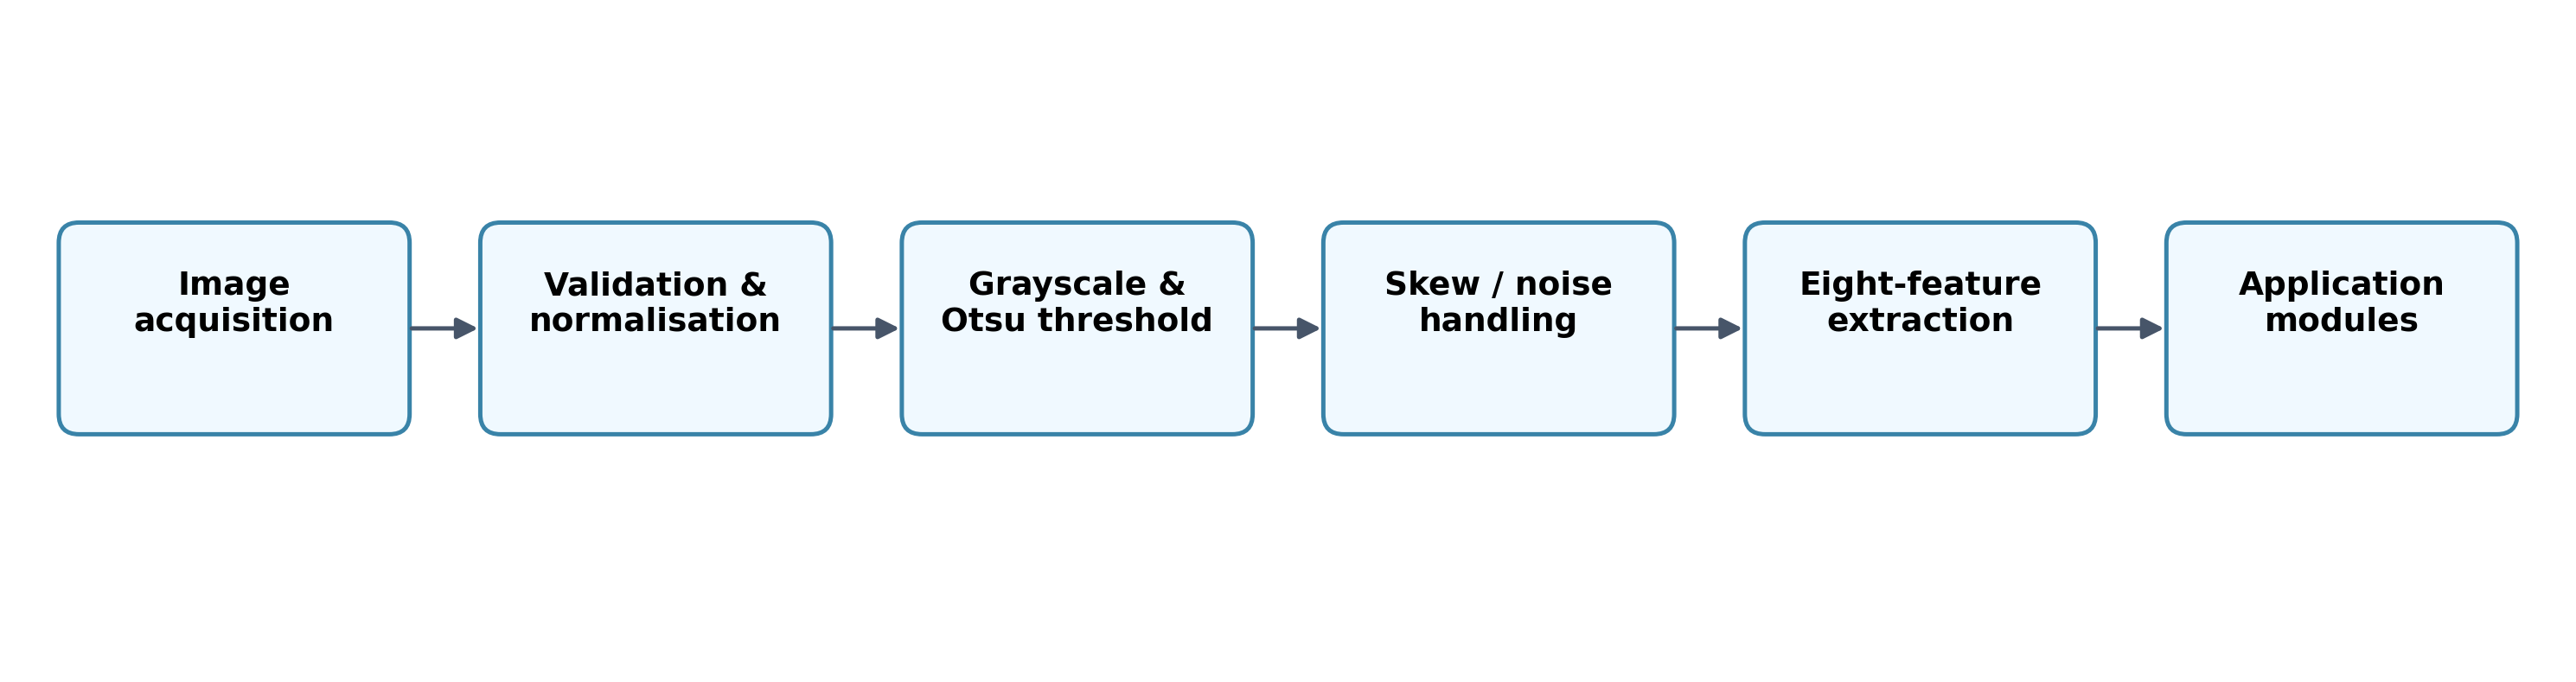
\includegraphics[width=\columnwidth]{paper_figures/fig2_workflow.png}
  \caption{Handwriting image processing and application workflow.}
  \label{fig:workflow}
\end{figure}

\begin{figure}[htbp]
  \centering
  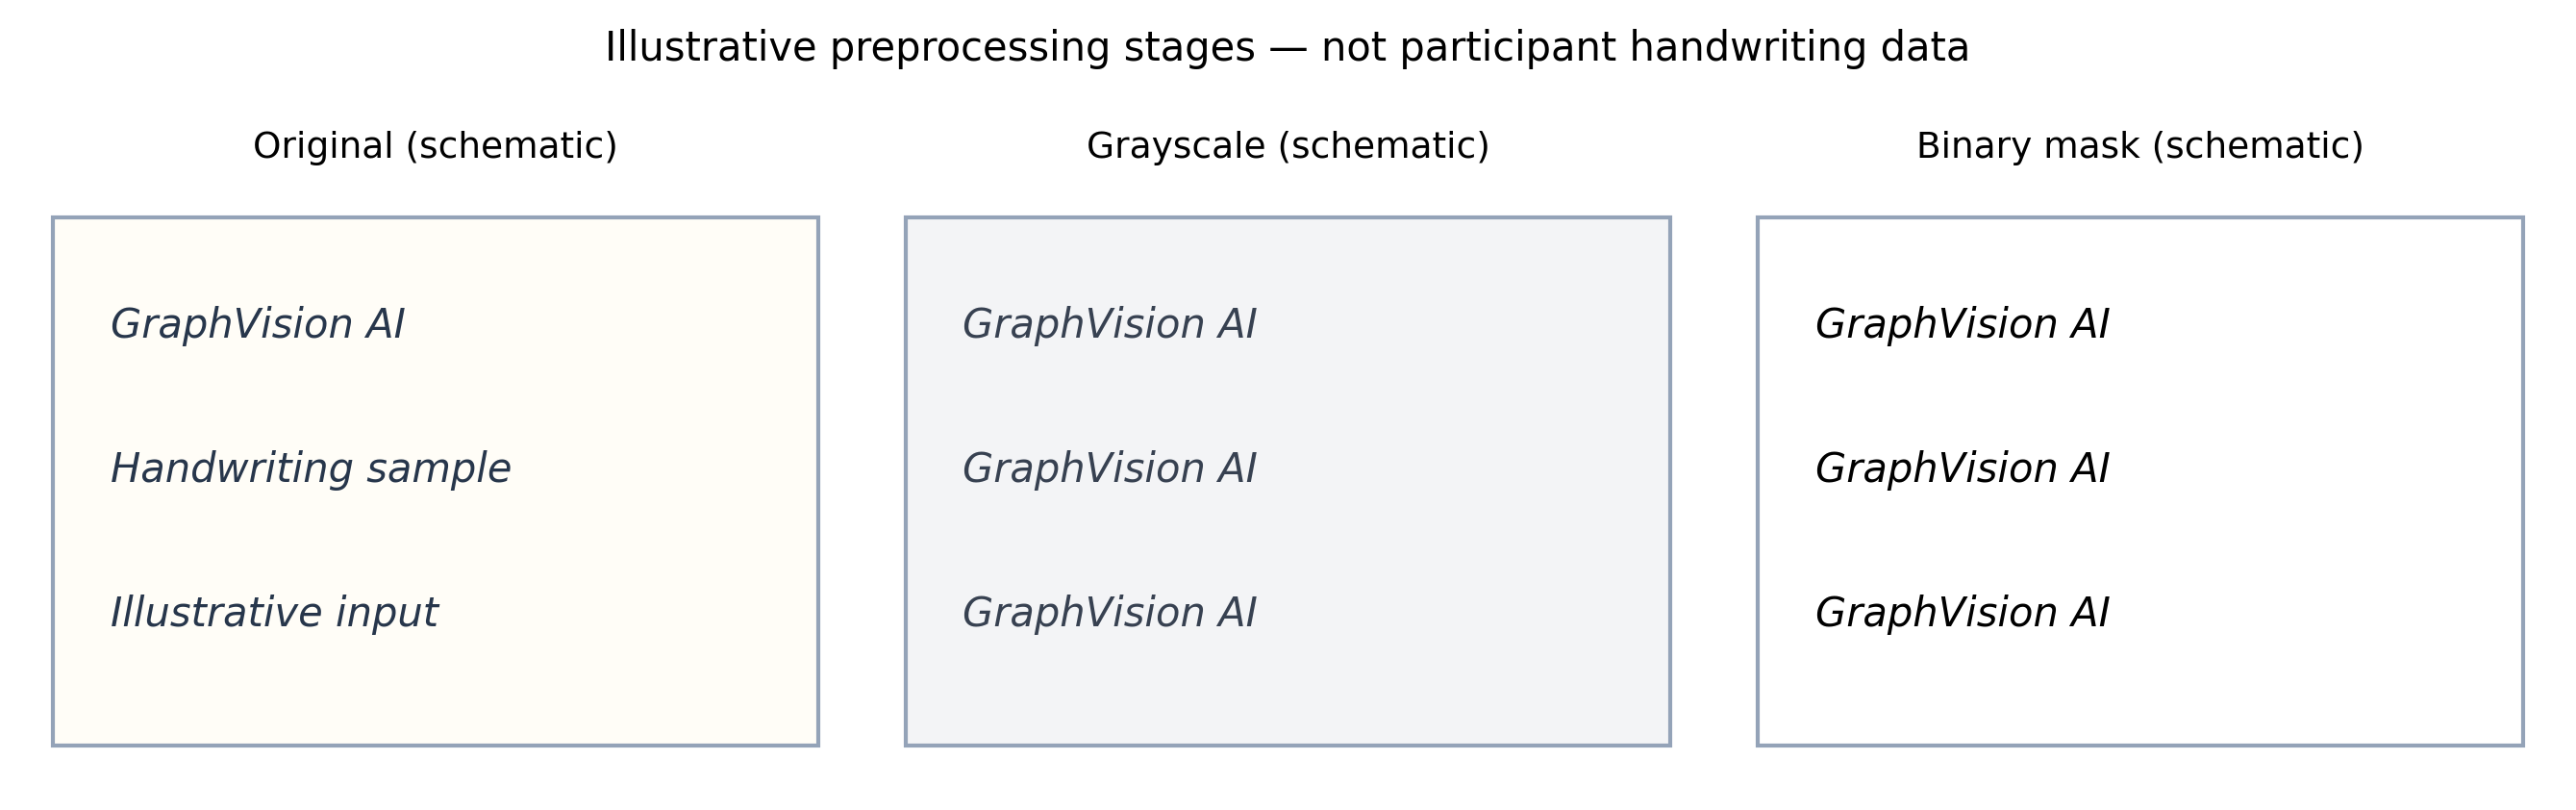
\includegraphics[width=\columnwidth]{paper_figures/fig3_preprocessing_schematic.png}
  \caption{Illustrative preprocessing stages (schematic; not participant data).}
  \label{fig:preprocessing}
\end{figure}

\begin{figure}[htbp]
  \centering
  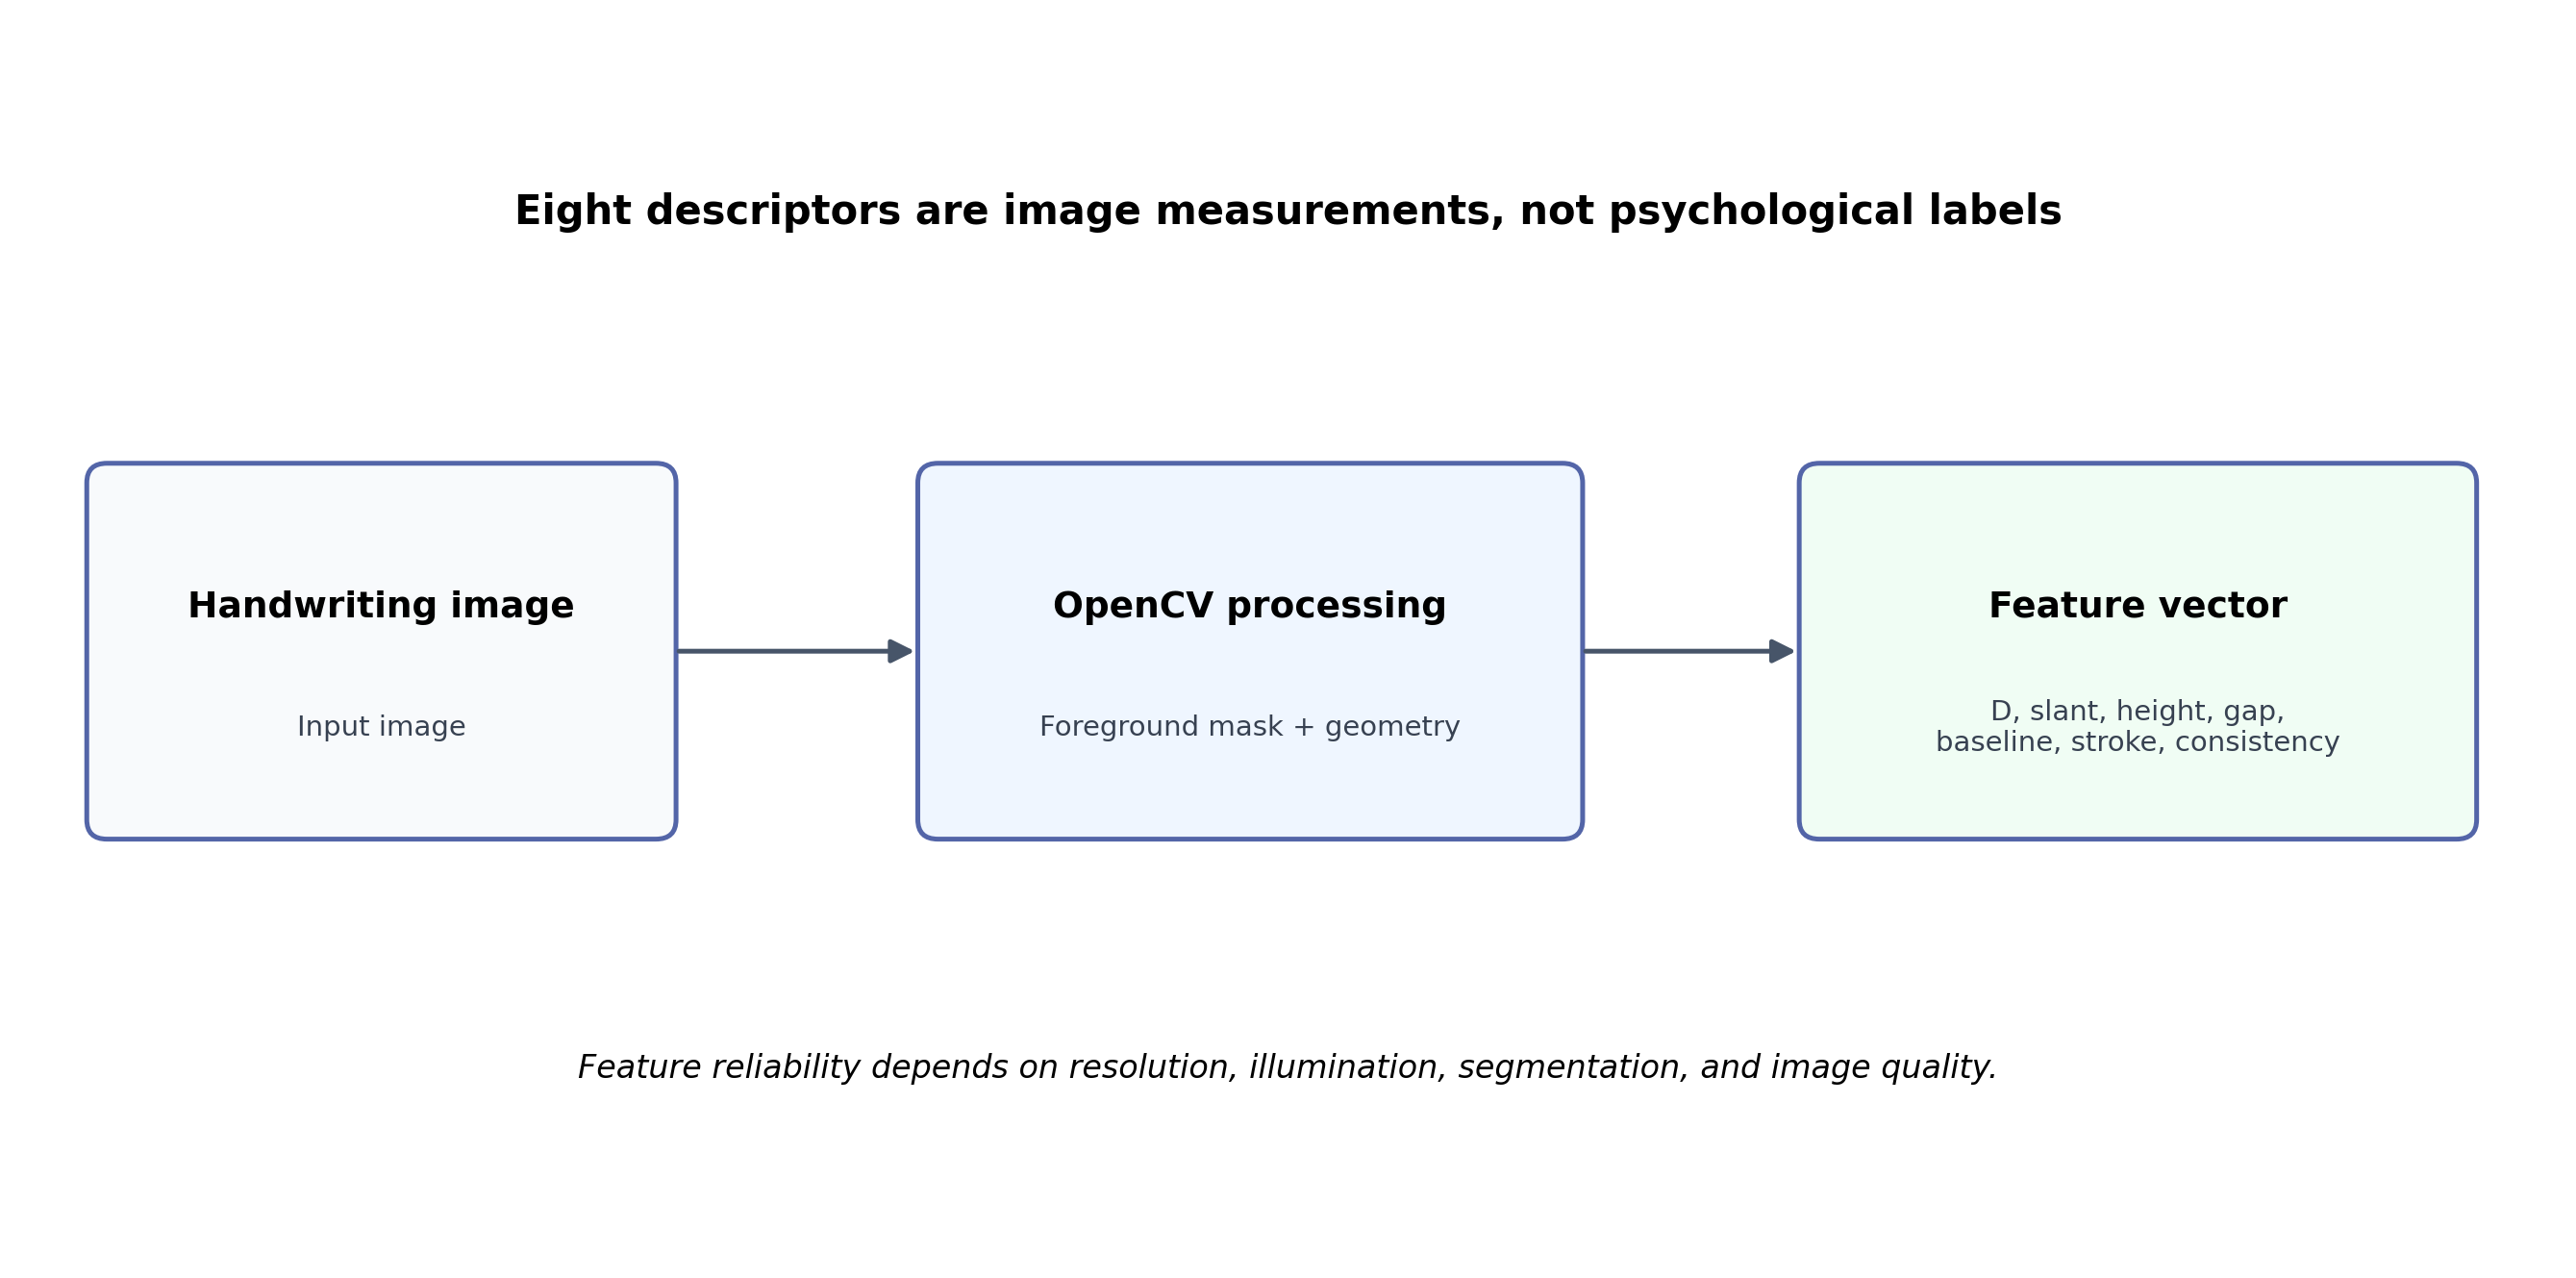
\includegraphics[width=\columnwidth]{paper_figures/fig4_feature_extraction.png}
  \caption{Conceptual representation of the eight-feature extraction process.}
  \label{fig:feature-extraction}
\end{figure}

\begin{figure}[htbp]
  \centering
  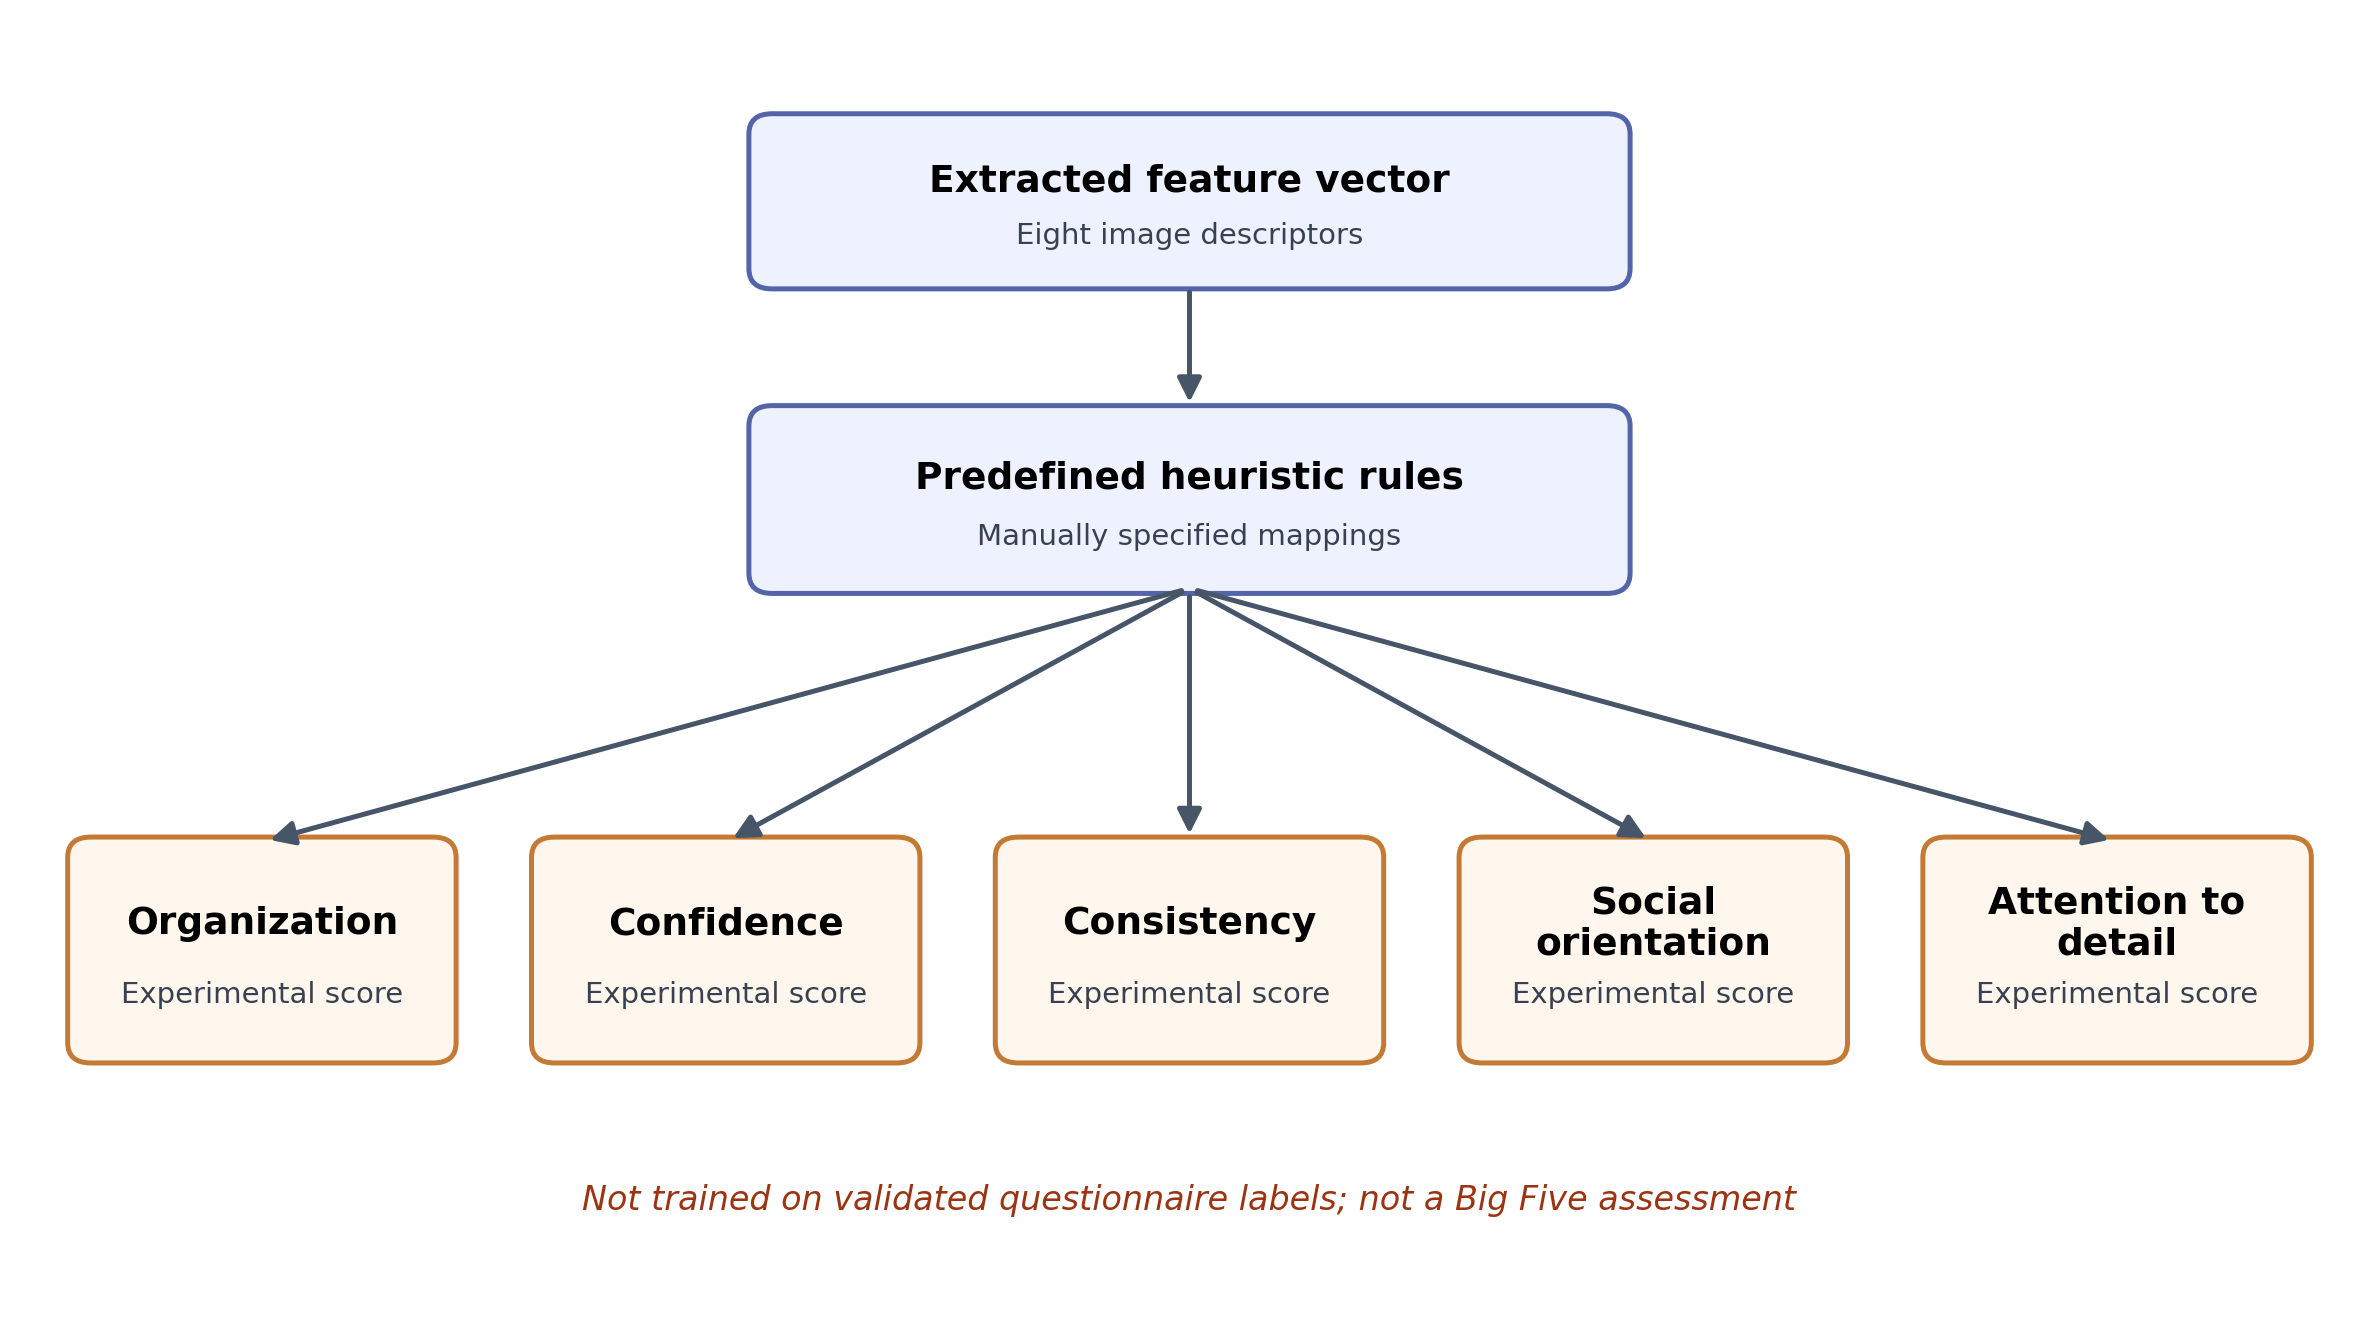
\includegraphics[width=\columnwidth]{paper_figures/fig5_personality_workflow.png}
  \caption{Conceptual workflow of the experimental personality association module.}
  \label{fig:personality-workflow}
\end{figure}

\begin{figure}[htbp]
  \centering
  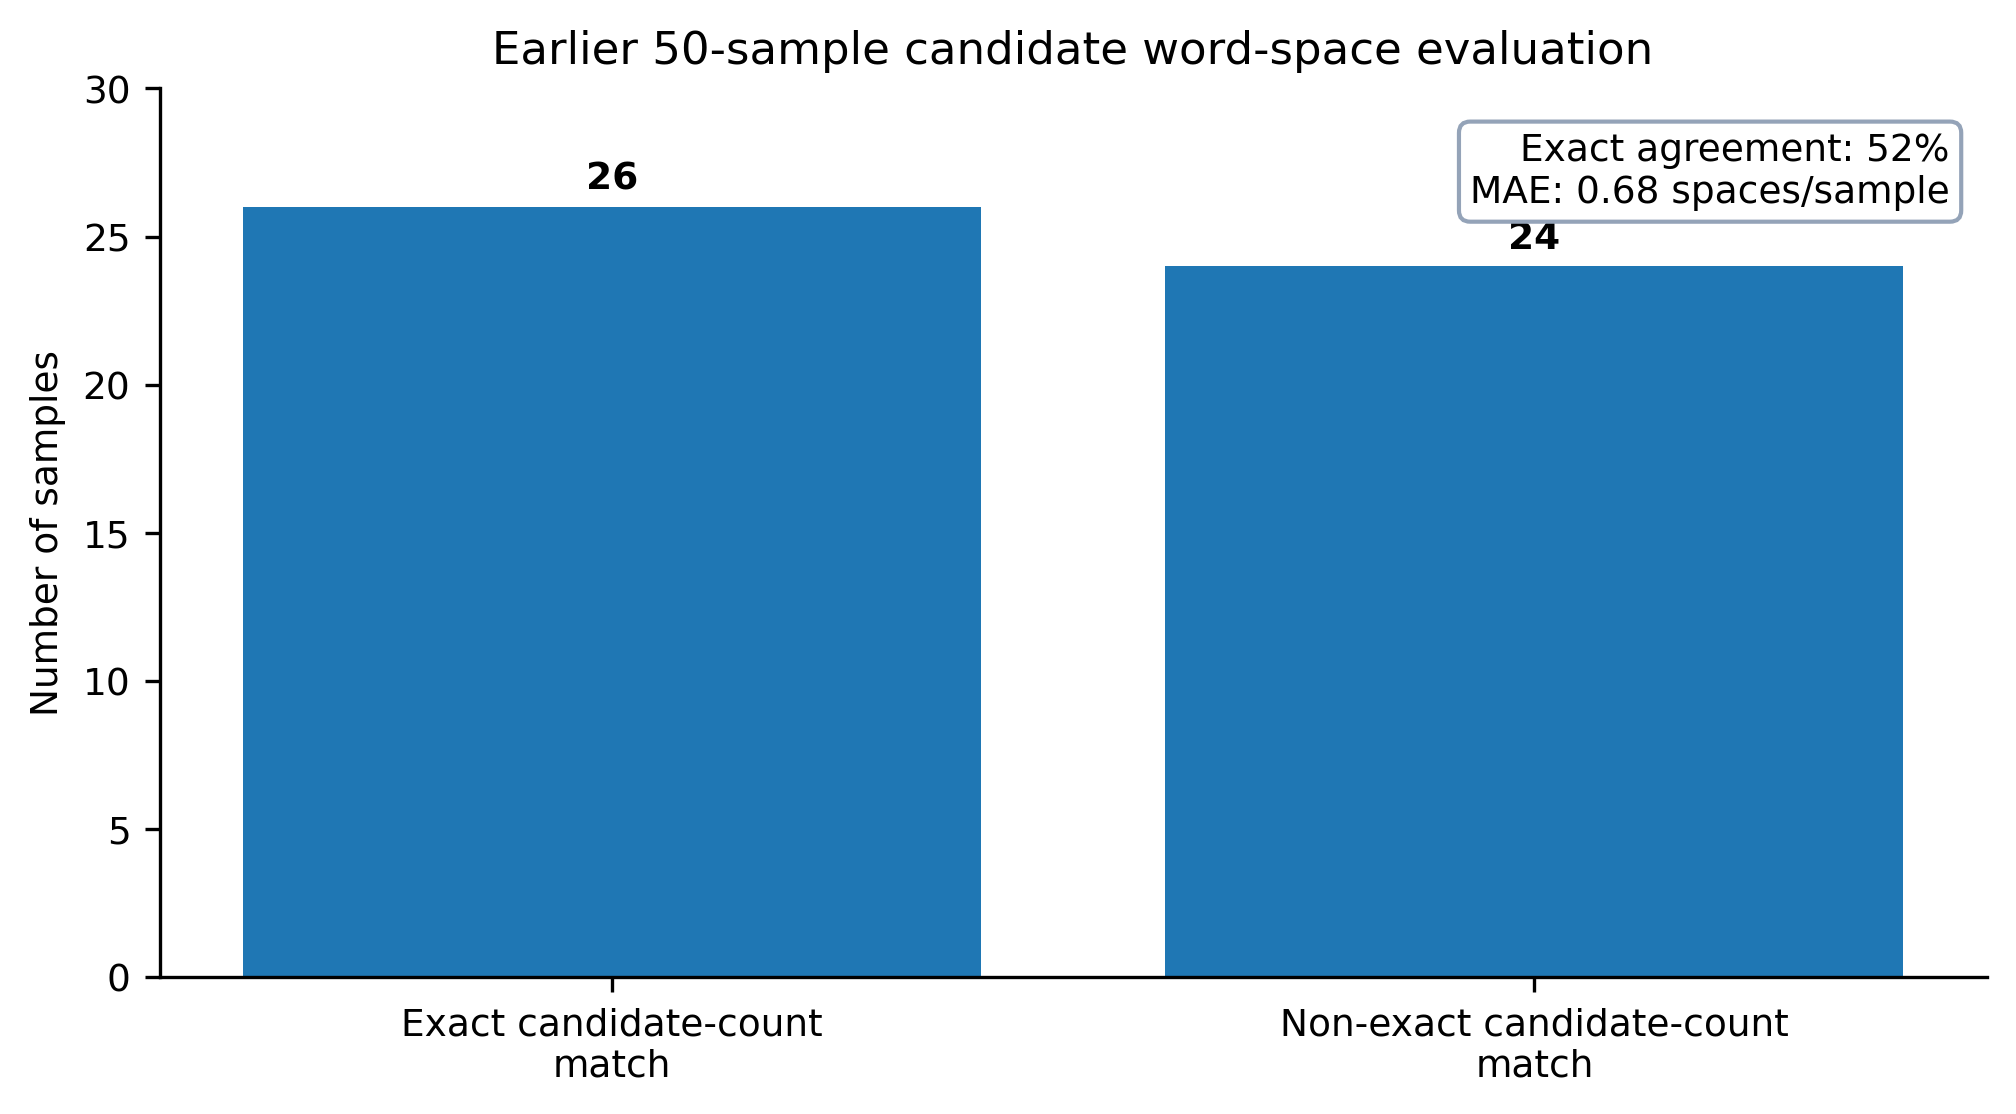
\includegraphics[width=\columnwidth]{paper_figures/fig6_wordspace_results.png}
  \caption{Earlier 50-sample candidate word-space count evaluation.}
  \label{fig:wordspace-results}
\end{figure}

\begin{figure}[htbp]
  \centering
  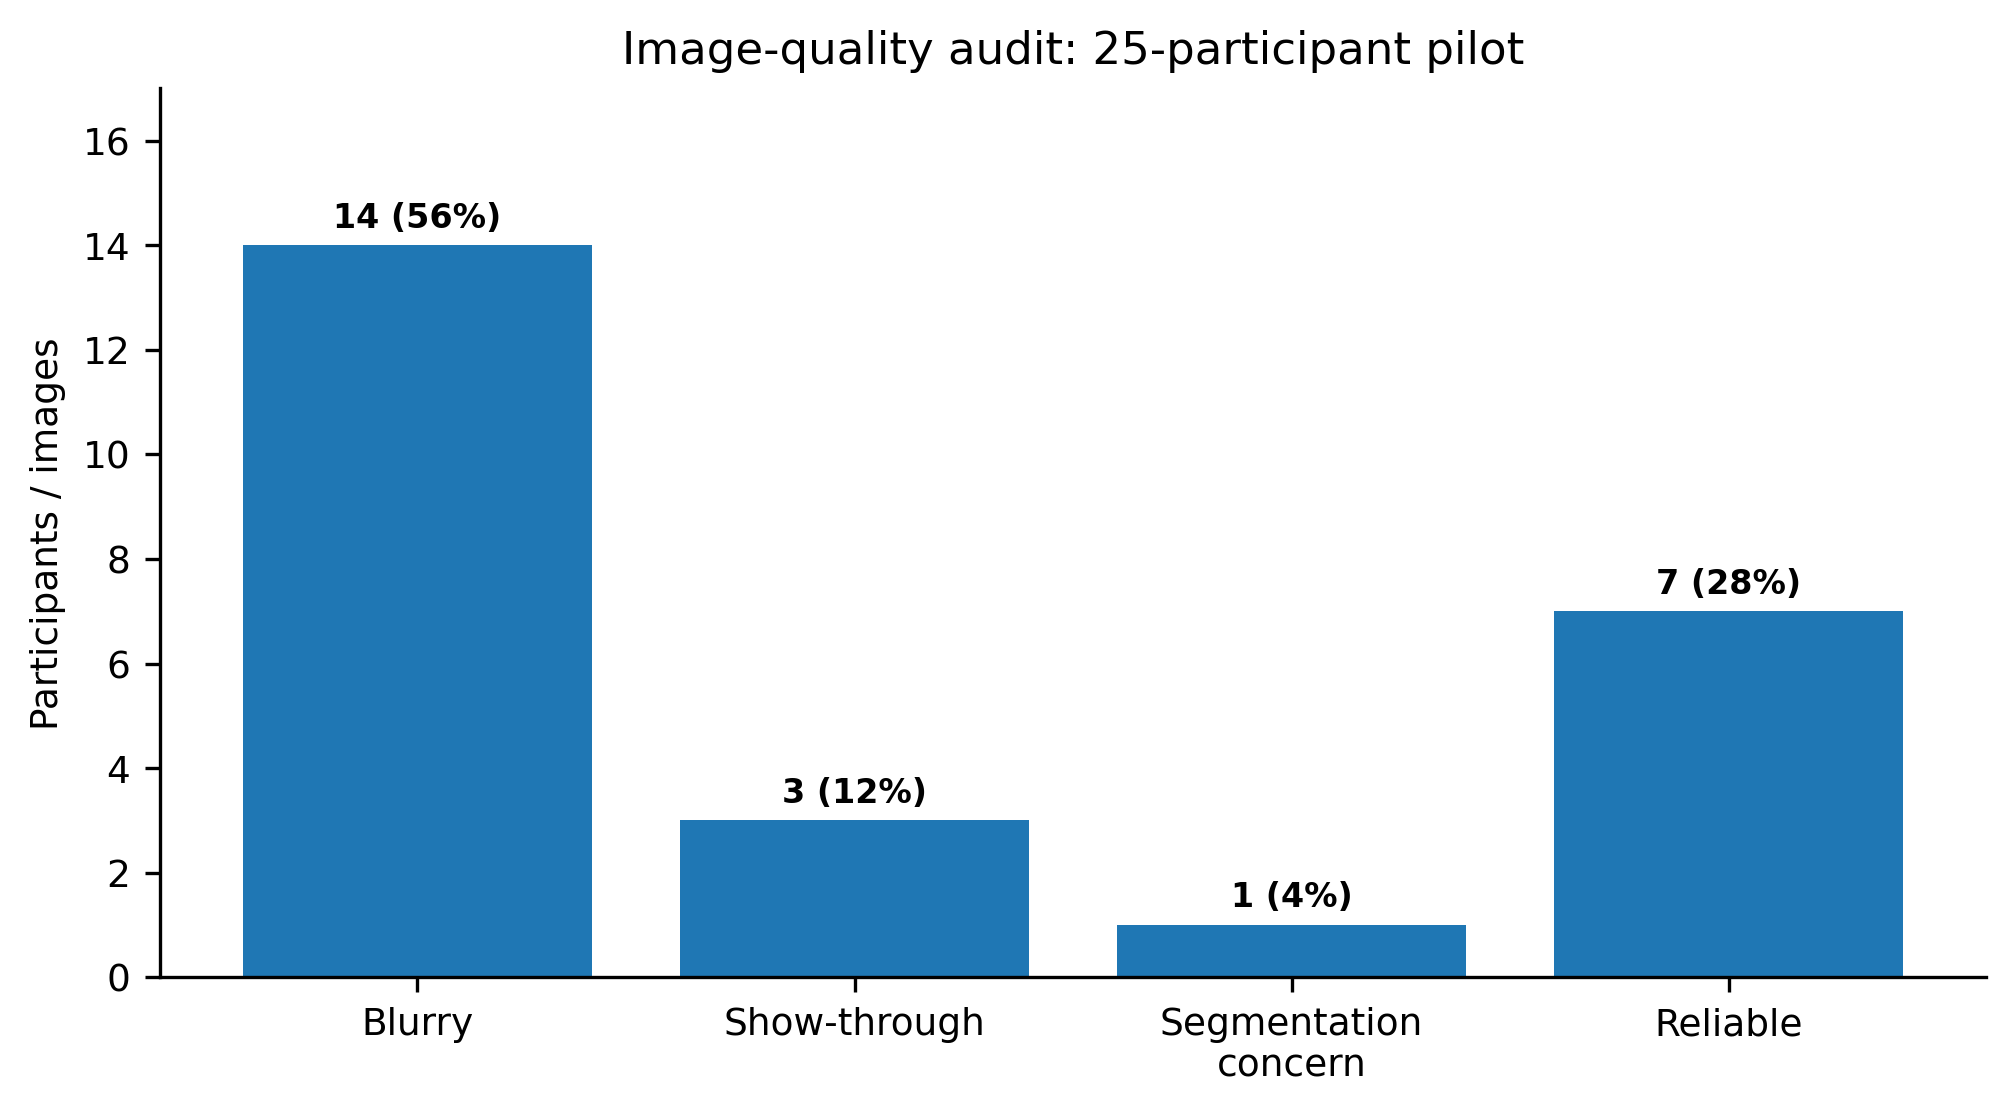
\includegraphics[width=\columnwidth]{paper_figures/fig7_pilot_quality.png}
  \caption{Image-quality distribution in the 25-participant pilot dataset.}
  \label{fig:pilot-quality}
\end{figure}

\begin{figure}[htbp]
  \centering
  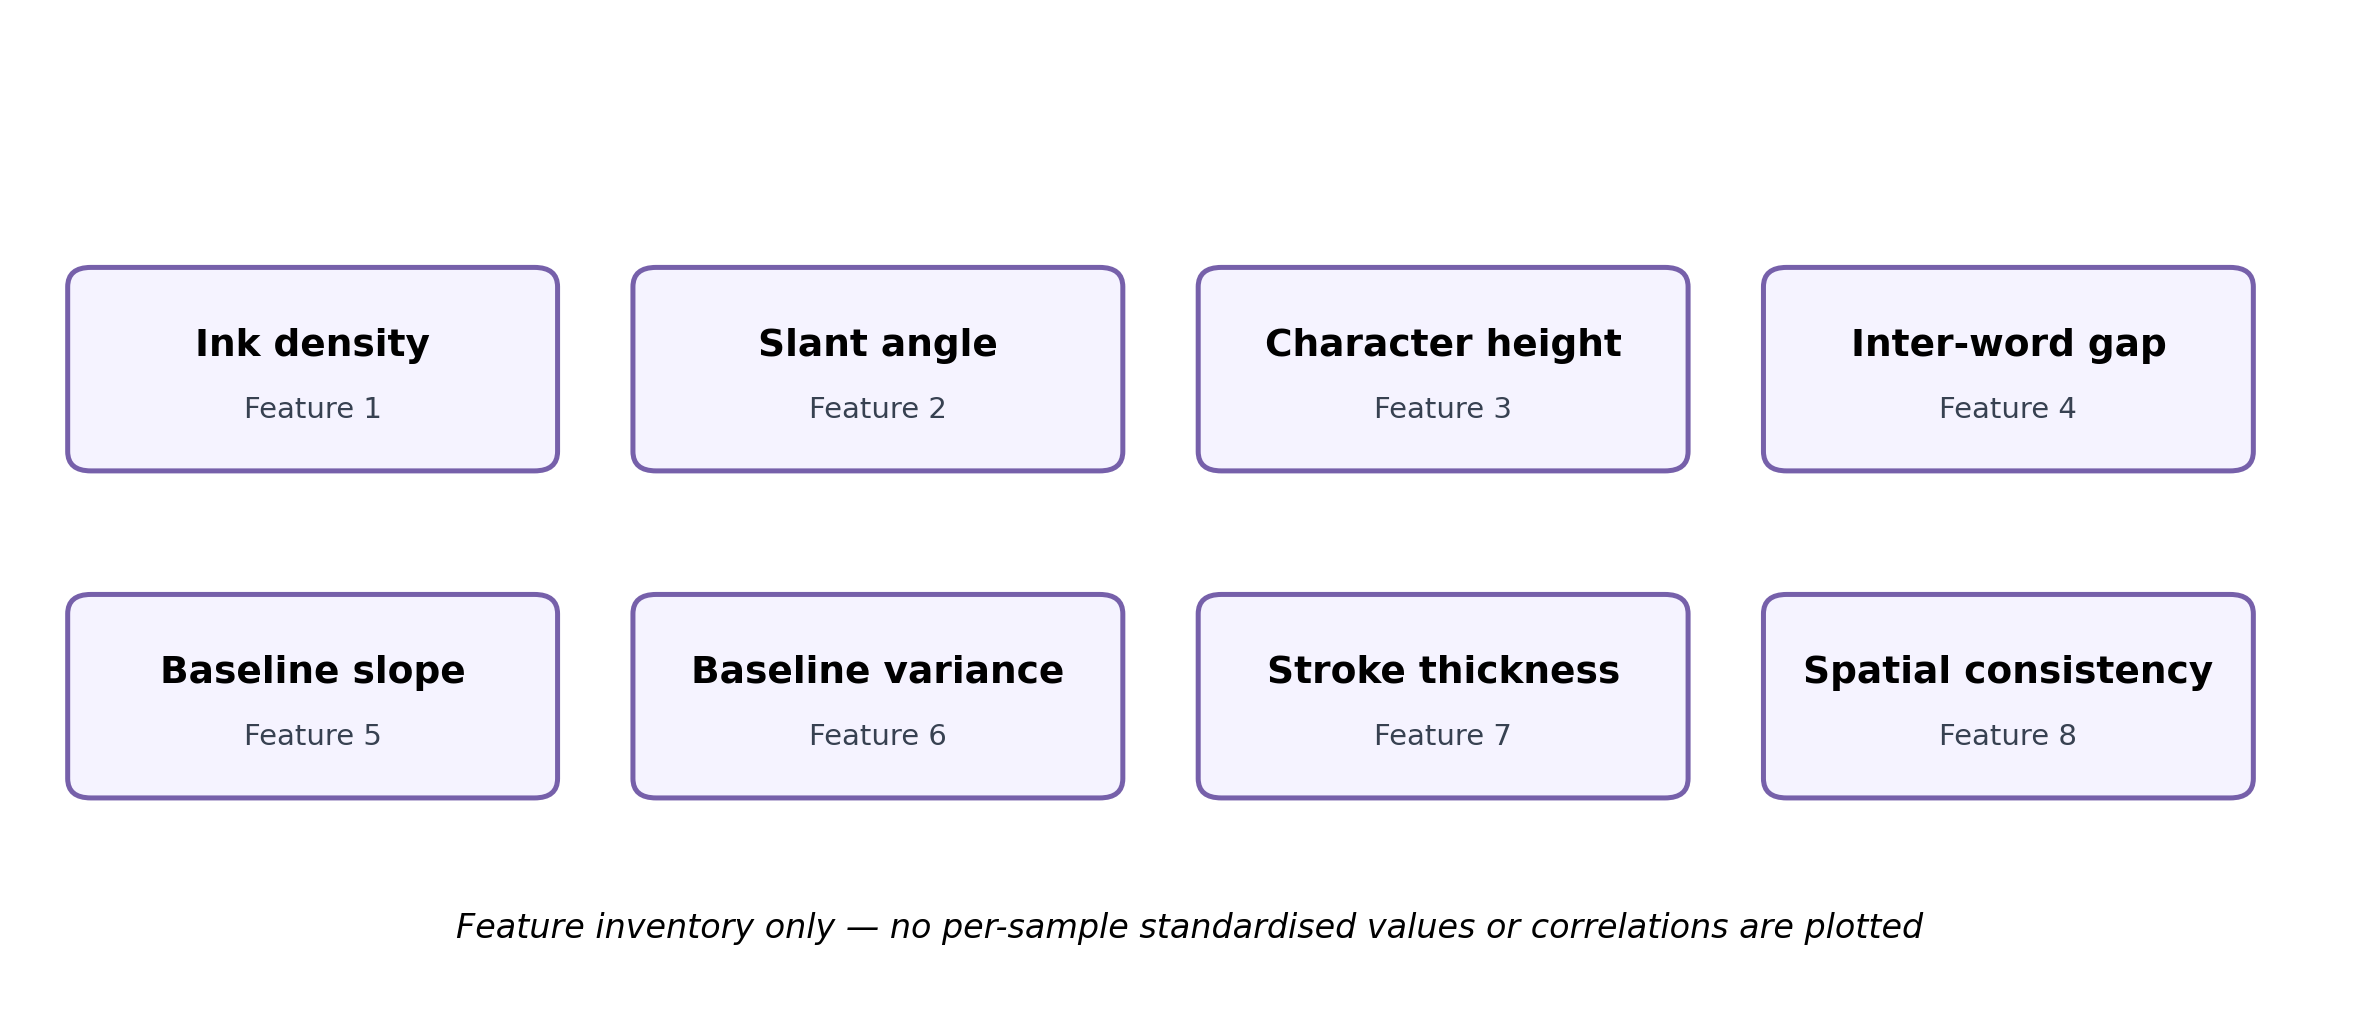
\includegraphics[width=\columnwidth]{paper_figures/fig8_feature_inventory.png}
  \caption{Inventory of the eight handwriting-image descriptors.}
  \label{fig:feature-inventory}
\end{figure}
